\section{METHODS PIPELINES}
\label{METHODS PIPELINES}

We reimplemented CNN from \cite{Feng2017} with one difference: we used squared pictures as an input, so we didn't implement Normalization layer (first layer in the Fig.~\ref{ris:CNN_feng2017}).
\begin{figure}[ht]
	\center{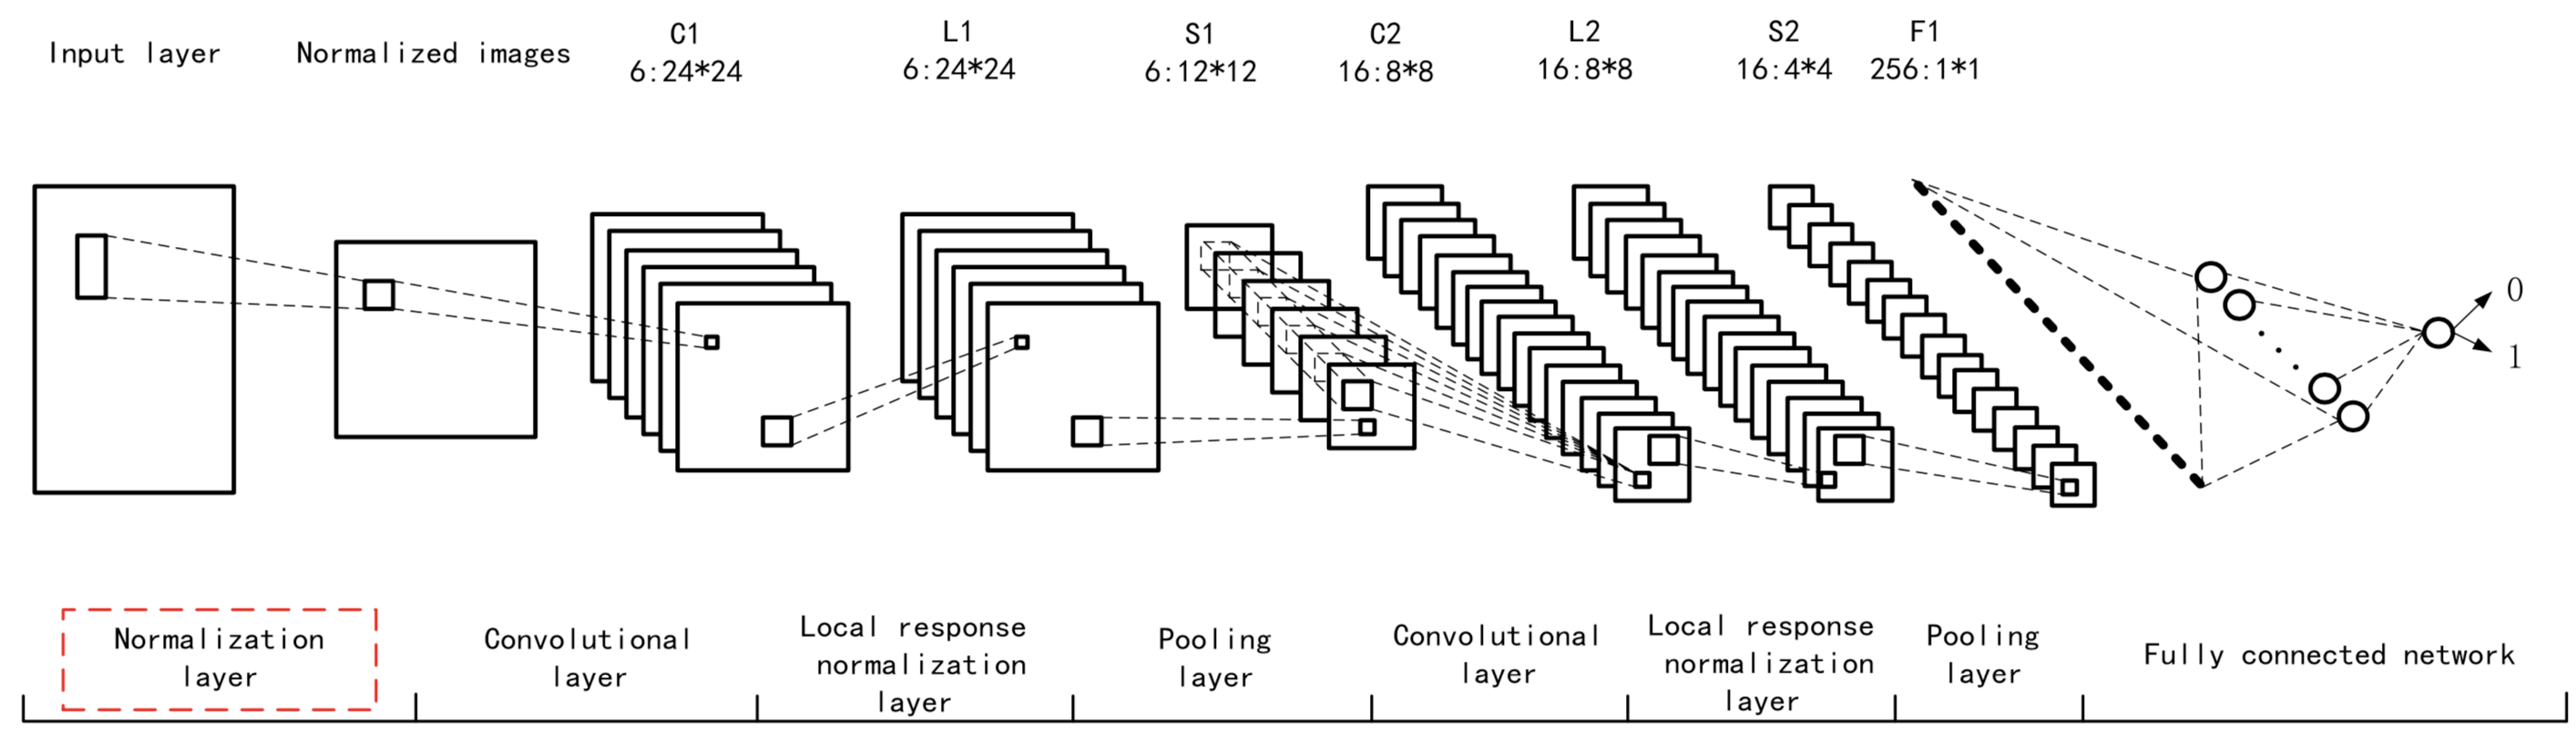
\includegraphics[scale=0.25]{pictures/CNN_feng2017.png}}
	\caption{Architecture of CNN from \cite{Feng2017}}
	\label{ris:CNN_feng2017}
\end{figure}

Our model contains Batch Normalization layers instead of Local Response Normalization layers and Dropout.
It consists of 5 Convolutional layers overall.
\begin{figure}[ht]
	\center{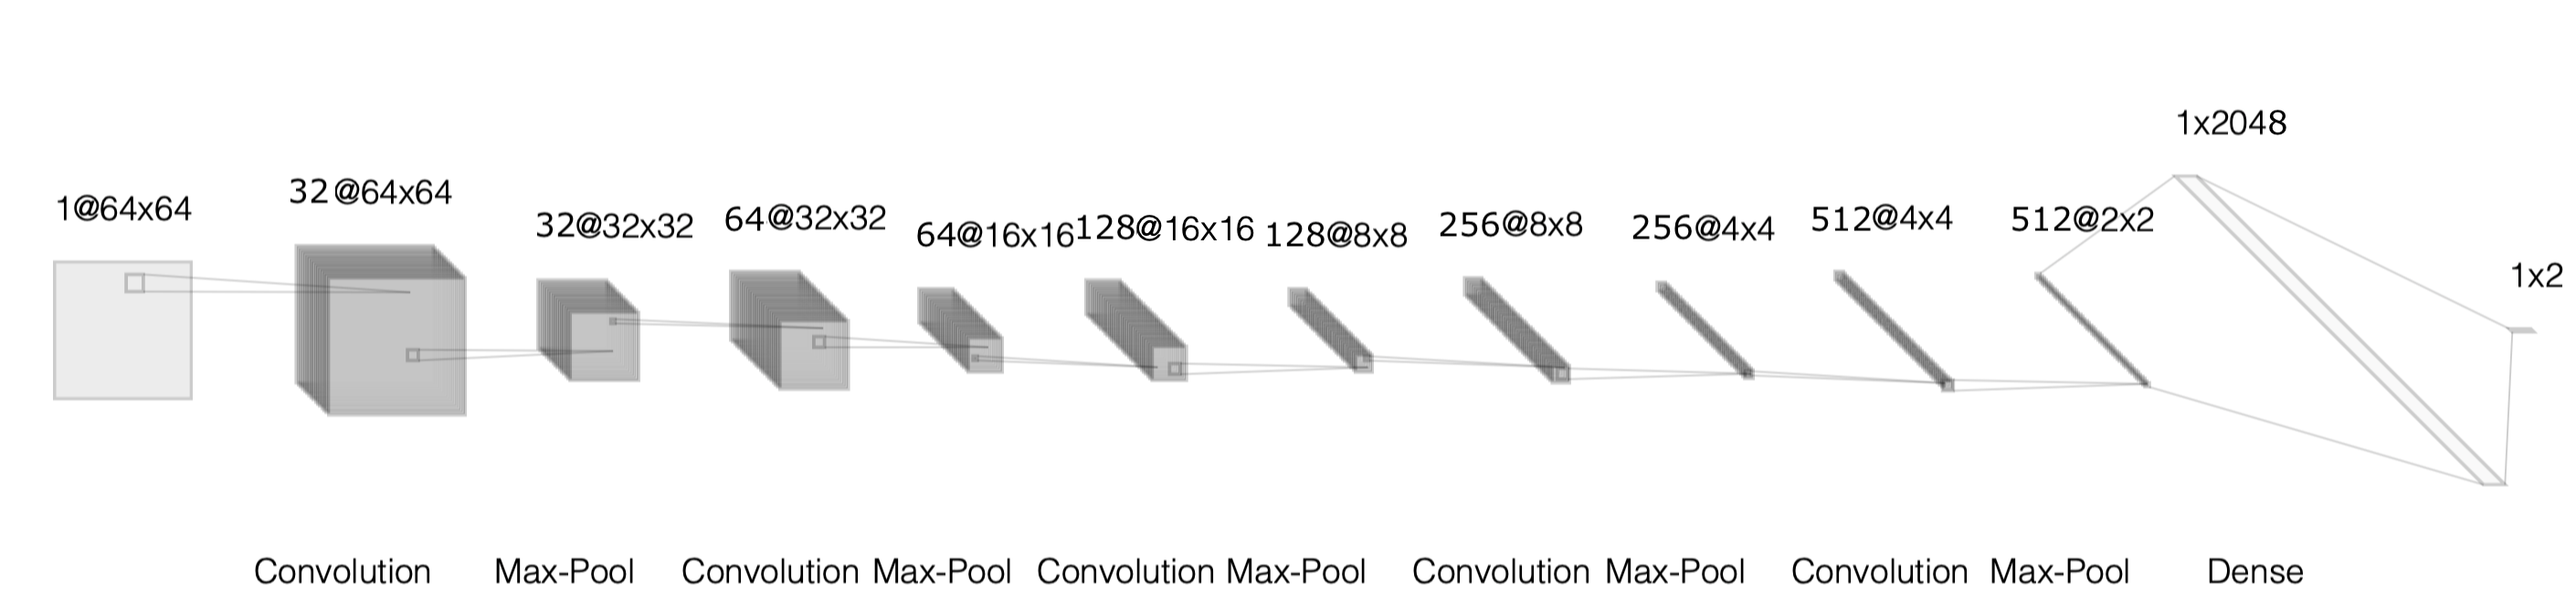
\includegraphics[scale=0.25]{pictures/CNN_our.png}}
	\caption{Architecture of our CNN}
	\label{ris:CNN_our}
\end{figure}

Batch size is equal to 64, so the input to the network has shape (64, 1, 64, 64).
For all experiments we use Adam optimizer with initial learning rate 0.001 and Learning Rate scheduler with parameters: threshold=0.0001, factor=0.5, min lr=0.0001, patience=484.
Also for all experiment the number of the epochs is equal to 12.

\subsection{Data and preprocessing description}
Although MFL data looks quite similar for different pipes and ILI tool types, it can differ a lot.
The data mainly depends on pipe size, wall width, sensors geometry and other geometric characteristics.
Moreover, the ILI tools differ a lot for different pipe sizes.
We have a data from the 219 mm in diameter pipe.
%Example of data is shown in Fig.~\ref{ris:data_example}.
%
%\begin{figure}[ht]
%	\center{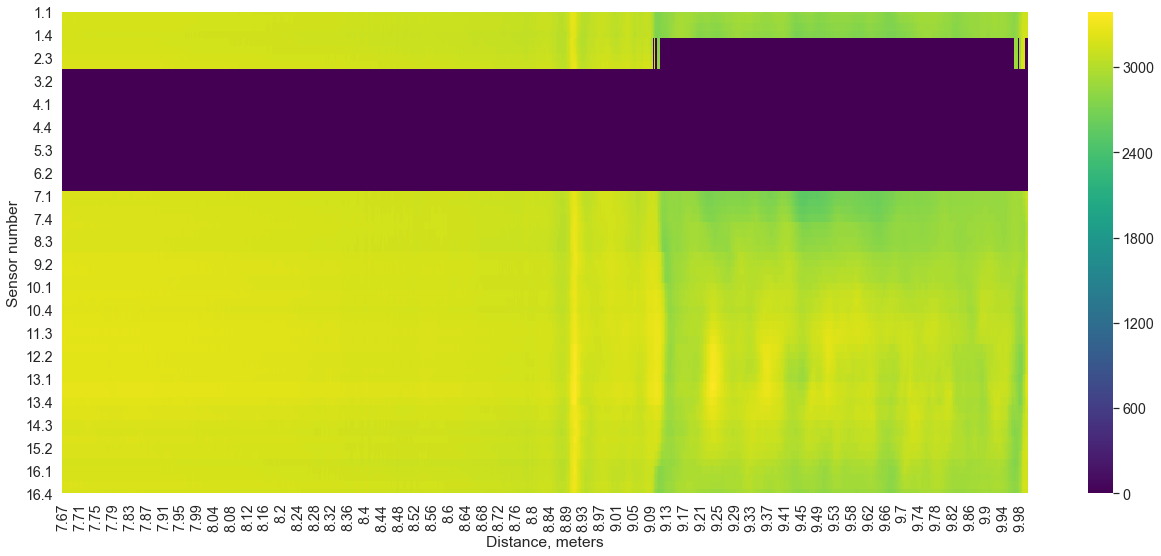
\includegraphics[scale=0.3]{pictures/0.png}}
%	\caption{Example of the MFL data}
%	\label{ris:data_example}
%\end{figure}
MFL dataset provides information about single inspection tool run.
Dataset has 64 features collected as an array with a constant step along the ILI tool movement inside the pipe.
Dataset has 4470704 samples that represent 15162.85 meters long pipeline part.
It has 745 defects of different types and 1462 welds.
Fig.~\ref{ris:defect_example} shows examples of normal data, data with a weld and with a defect.
Attached to the dataset technical report contains information about welds and defects location, defects types, sizes and other related characteristics.
\begin{figure}[ht]
	\center{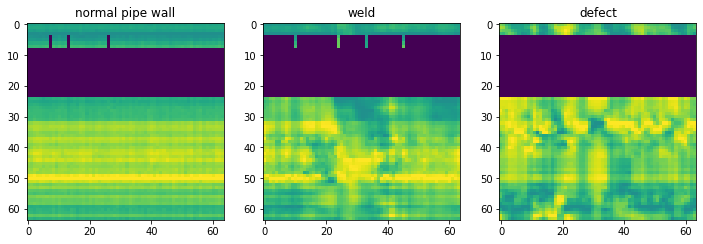
\includegraphics[scale=0.55]{pictures/1.png}}
	\caption{Example of the MFL data}
	\label{ris:defect_example}
\end{figure}

Raw data has several issues that don't allow to solve CV problems without proper preprocessing.
They are:
\begin{enumerate}
	\item Sensors malfunctions (zeroed values cause bold horizontal line in Fig.~\ref{ris:defect_example});
	\item Displaced origins between data and report files coordinates;
	\item Inaccurate annotations, e.g. missed defect, wrong defect location, etc.
\end{enumerate}

In addition to preprocessing, data were annotated for the segmentation task.

\subsubsection{Sensors malfunctions problem}
To deal with sensors malfunctions we suppose to fill the gaps (zeroed values) with values calculated by different methods:
\begin{enumerate}
	\item Scaling of picture values to $[0.5:1]$ range. Abnormal values ($<2000$) are equal to 0.
	\item Abnormal values are equal to the mean of normal values from one picture.
	\item Abnormal values are equal to the mean of normal values over the column.
	\item Abnormal values are equal to the mean of neighboring sensors over the column.
	\item Abnormal values are equal to the interpolation results over the column.
	\item Rerange initial set of values to 0...255 uint8 range.
	\item Rerange initial set of values to 0...1 float range.
	
	
\end{enumerate}
The results of all applied methods are presented in Fig.~\ref{ris:filling_example}.
\begin{figure}[ht]
	\center{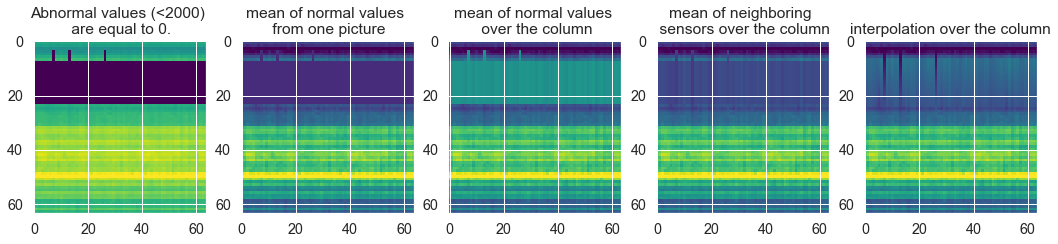
\includegraphics[scale=0.4]{pictures/2.png}}
	\caption{The results of missing values filling methods}
	\label{ris:filling_example}
\end{figure}

\subsubsection{Displaced origins problem}

Since the data on the location of the robot did not match the defect location data from the report, it was necessary to merge the data. The key factor here turned out to be that the values of signal from magnetic flux sensors grow at the weld site, see picture \ref{ris:prepr}. 

\begin{figure}[!h]
	\center{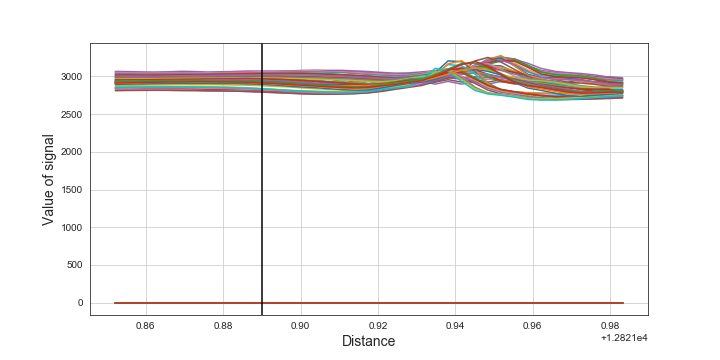
\includegraphics[width=0.8\linewidth]{pictures/prepr.png}}
	\caption{Location of weld. Black vertical line in accordance with defect location data from the report. Others lines are values from sensors.}
	\label{ris:prepr}
\end{figure}
The locations of maxima of these values have been founded and then combined with welds locations.


\subsubsection{Inaccurate annotations problem}
This problem is a common one for oil and gas pipeline nondestructive testing \cite{Khodayari-Rostamabad2009}.
It appears to be a lot of missing defects that affects the quality of the problem.
Besides there are wrong defect type and locations.
For wrong location issue elimination we additionaly searched extremums around the provided location and chose the defects or welds taking into account new coordinates.

\subsubsection{Augmentation}
Although we have a lot of data, we don't have a lot of defects and welds in comparison with normal pipe wall instances.
We use augmentation procedure to balance classes of pictures and increase model's quality by increasing number of instances in small classes (defects, welds).
As an augmentation tool we use Albumentations library \cite{buslaev2020albumentations}.
For welds pictures we apply following augmentations:
\begin{enumerate}
	\item Rotate (limit=180, p=1),
	\item VerticalFlip (p=1), 
	\item HorizontalFlip (p=1), 
	\item ElasticTransform (p=1, alpha=20, sigma=120 * 0.05, alpha affine=120 * 0.03), 
	\item GridDistortion (p=1),
	\item OpticalDistortion (p=1, distort limit=2, shift limit=0.5).
\end{enumerate}

And for defects we apply following ones:
\begin{enumerate}
	\item Transpose (p=1), 
	\item Rotate (limit=90, p=1), 
	\item Rotate (limit=180, p=1), 
	\item Rotate (limit=270, p=1,), 
	\item VerticalFlip (p=1), 
	\item HorizontalFlip (p=1), 
	\item ElasticTransform (p=1.0, alpha=20, sigma=120 * 0.05, alpha affine=120 * 0.03),
	\item RandomRotate90 (p=1.0),
	\item GridDistortion (p=1.0),
	\item OpticalDistortion (p=1, distort limit=1, shift limit=0.3).
\end{enumerate}
Examples of augmentations are shown in Fig.~\ref{ris:aug_example}.
\begin{figure}[ht]
	\center{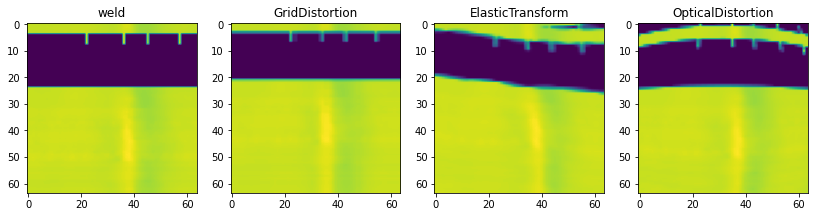
\includegraphics[scale=0.55]{pictures/4.png}}
	\caption{Examples of the augmentation results}
	\label{ris:aug_example}
\end{figure}


\begin{table}[!htb]
	\caption{\label{tab:alg1}Dataset size for pipeline defects detection and segmentation problems}
	\begin{center}
		\small
		\begin{tabular}{| l | c | c | c |}
			\multicolumn{1}{c}{} & \multicolumn{3}{c}{Classification} \\
			\hline
			Data& Normal pipe wall & Defect & Weld \\
			\hline
			\multicolumn{4}{|c|}{Before augmentation}  \\
			\hline
			Train  & 11106 & 1130 & 569 \\
			Validation & 584 & 282 & 142 \\
			\hline
			\multicolumn{4}{|c|}{After augmentation}  \\
			\hline
			Train  & 11106 & 11300 & 8535 \\
			Validation & 584 & 282 & 142 \\
			\hline
		\end{tabular}
	\end{center}
\end{table}

\subsection{Performance metrics}
For the classification problem we use Accuracy.
Accuracy is defined by the formula:
$$Acc = \frac{\sum_{i=0}^{N} 1_{\{\hat{y}_i=y_i\}}}{N},$$
where $N$ - number of samples, $\hat{y}$ - predicted label, $y$ - true label.
